\documentclass[conference]{IEEEtran}
\usepackage[utf8]{inputenc} % To use Unicode (e.g. Turkish) characters
\usepackage[T1]{fontenc}
\renewcommand{\labelenumi}{(\roman{enumi})}
\usepackage{amsmath, amsthm, amssymb}
 % Some extra symbols
\usepackage[bottom]{footmisc}
\usepackage{cite}
\usepackage{graphicx}
\usepackage{url}
\usepackage{multicol}
\usepackage{longtable}
\graphicspath{{figs/}} % Graphics will be here

\usepackage{multirow}
\usepackage{subcaption}
\usepackage[linesnumbered,ruled,vlined]{algorithm2e}

\usepackage{soul}
\usepackage[dvipsnames]{xcolor}
\DeclareRobustCommand{\fba}[1]{ {\begingroup\sethlcolor{BurntOrange}\hl{(fba:) #1}\endgroup} }
\DeclareRobustCommand{\sgk}[1]{ {\begingroup\sethlcolor{Yellow}\hl{(sgk:) #1}\endgroup} }
\begin{document}


\title{A Requirement Traceability Tool: ABV}
\author{
 \IEEEauthorblockN{Kadir Ersoy, Ecenur Sezer, Suzan Üsküdarlı, Fatma Başak Aydemir}
\IEEEauthorblockA{
Boğaziçi University\\
Istanbul, Türkiye \\
\{kadir.ersoy, ecenur.sezer, suzan.uskudarli, basak.aydemir\}@boun.edu.tr}
}

\date{May 2021}

\maketitle
\begin{abstract}
    Requirements traceability refers to the capability of following the life of a requirement in both forwards and backward directions, and to the ability to link requirements to other software artifacts through particular relationships. These traceability links enable stakeholders to monitor the development progress of requirements and assist system engineers in tracking the effort and workload associated with fulfilling those requirements. Traditional methods to recover traceability links necessitate significant human effort, making them unsuitable and inefficient, particularly as the project scale grows. In this work, we present a tool that establishes automated requirement traceability links between requirements written in natural language and software artifacts acquired from GitHub repositories. The tool implements three optional methods to trace the artifacts to the requirements, namely a keyword extraction pipeline, TF-IDF vector and word-vector. The captured traces are stored in a graph database and visualized. Additionally, an interactive dashboard featuring statistical data about the artifacts and their traces is implemented. By offering automated traceability and comprehensive visualization, this tool aims to enhance the management of requirements and to understand their quality in software development projects.
\end{abstract}
\begin{IEEEkeywords}
Requirement traceability, NLP, Keyword extraction, Traceability graph
\end{IEEEkeywords}

\section{Introduction} \label{section:introduction}

% \begin{itemize}
%     \item Requirements traceability definition
%     \item Why do we do it, examples
%     \begin{itemize}
%         \item It is too hard to do it manually
%         \begin{itemize}
%             \item Cost of integration: Need trace link recovery, 
%             \item Human effort: Do not force extra measures for traceability
%         \end{itemize}
%         \item Its role in project management
%         \begin{itemize}
%             \item Monitoring the progress: Status of the project
%             \item Effort assessment: How much effort went to which features
%             \item Detecting problems for specific features
%         \end{itemize}
%     \end{itemize}
%     \item showcasing trace data and other stats to user in a self-evident manner
% \end{itemize}

Requirements traceability refers to the capability of following the life of a requirement in both forwards and backward directions\cite{gotel-1994}, and to the ability to link requirements to other software artifacts through particular relationships. Requirement traceability is crucial in software development projects since it shows the progress done in implementing the requirements and assists engineers in observing the effort and workload associated with them. All these aspects of requirement traceability help teams to ensure the fulfillment of specified requirements, by linking them to other software artifacts. Given that, it is a critical obstacle that traditional methods of recovering traceability links require significant time and human effort, making them unsuitable for the task as the project scale grows. Moreover, the quality of these methods is not consistent, since it highly depends on the understanding of the requirement traceability of the human analysts' performing them. 
In this paper, we present a tool implemented to automate the process of identifying trace links. Our tool establishes links from requirements that are written in natural language to the software development artifacts, mainly Issues, PRs, and Commits, that are fetched from GitHub repositories. By automatizing this process, our tool aims to decrease the reliance on human effort and provides efficient requirement traceability management.

For identifying the trace links, three optional methods are implemented in our tool. These methods are keyword extraction, which performs keyword matching to software development artifacts, and TF-IDF Vector - Word Vector methods, which basically perform vector-based similarity. Each of these methods offers distinct advantages that are highly dependent on the context of the projects.
The software artifacts and the identified trace links are stored in a graph database and visualized in a graphical structure to enable efficient retrieval of traceability information. To improve the comprehension of the collected traceability data, our tool also features an interactive dashboard. This dashboard is equipped with valuable statistical insights about the lifetime of the project and the requirements. Along with the visualization of the traceability links and the offering of statistical data, we aim to improve the management of the requirements, ultimately leading to better-planned and programmed software projects.

%\section{Problem and Motivation}
%\label{section:problem}

% Requirements traceability, 
%     - definition, 
% Why do we do it, examples
%     - It is too hard to do it manually
%     - Its role in project management,
%         - Monitoring the progress
%             - Status of the project
%             - What has been done 
%         - Effort assessment
%             - How much effort went to which features
%         - Detecting problems for specific features
%             - In the case of a problem, look for it in a localized manner 
%             - can be done since we know what has done for which context
%     - The use of requirements and req traceability is not common
%         - Cost of integration
%             - Need trace link recovery, 
%         - Human effort
%             - Do not force extra measures for traceability
%     - To achieve wide-use of traceability
%         - user friendly, 
%             - showcasing trace data and other stats to user in a self-evident manner
%         - minimal human effort, 


\section{Related Work}
\label{section:related_work}

There are several studies that focus on automatizing requirements traceability by implementing various techniques. Hayes et al. (2003)\cite{hayes-2003} have studied an approach that frames requirement traceability as an information retrieval(IR) problem. Their study aims to enhance recall and precision values of capturing traces. The IR methods they have implemented performed a significantly higher retrieval percentage, relative to the manual tracing. In a different study, Abdeen (2023)\cite{abdeen-2023} established a system that grips taxonomic trace links to link software development artifacts and requirements. In this approach, requirement artifacts are labeled with system-recommended labels based on their textual data. Bonner et al. (2023)\cite{bonner-2023} have developed a tool that performs Artificial Intelligence(AI) to identify trace links between requirements and model-based designs. They have integrated their tool into the Siemens toolchain for Application Lifecycle Management(ALM) and performed experiments on the traceability problem with the natural language requirements and system design models. Cleland-Huang et al. (2007)\cite{cleland-huang-2007} focused on nine best practices for implementing automated traceability. These practices include information retrieval methods, and they have significantly diminished the amount of effort given to produce a requirement trace matrix. Mills (2017)\cite{mills-2017} automated traceability link recovery(TLR) with machine learning algorithms and approached TLR as a binary classification problem.

These studies have integrated relatively more modern technologies such as artificial intelligence, machine learning, and information retrieval algorithms to automated trace links recovery and encouraged the researches to implement various approaches to minimize the effort and maximize the quality of requirement traceability.



\section{Method}
\label{section:method}
% \begin{itemize}
%     \item Inputs-outputs
%     \item Workflow + diagrams
%     \item Heuristics:
%     \begin{itemize}
%         \item Keyword extraction, more detailed than poster
%         \item Vector-based methods, more detailed than poster
%     \end{itemize}
%     \item Implementation:
%     \item \begin{itemize}
%         \item Trace graph + visuals
%         \item Dashboard
%         \item (Using same example for trace finding and trace graph)
%     \end{itemize}
% \end{itemize}

\begin{figure}[htb]
    \centering
    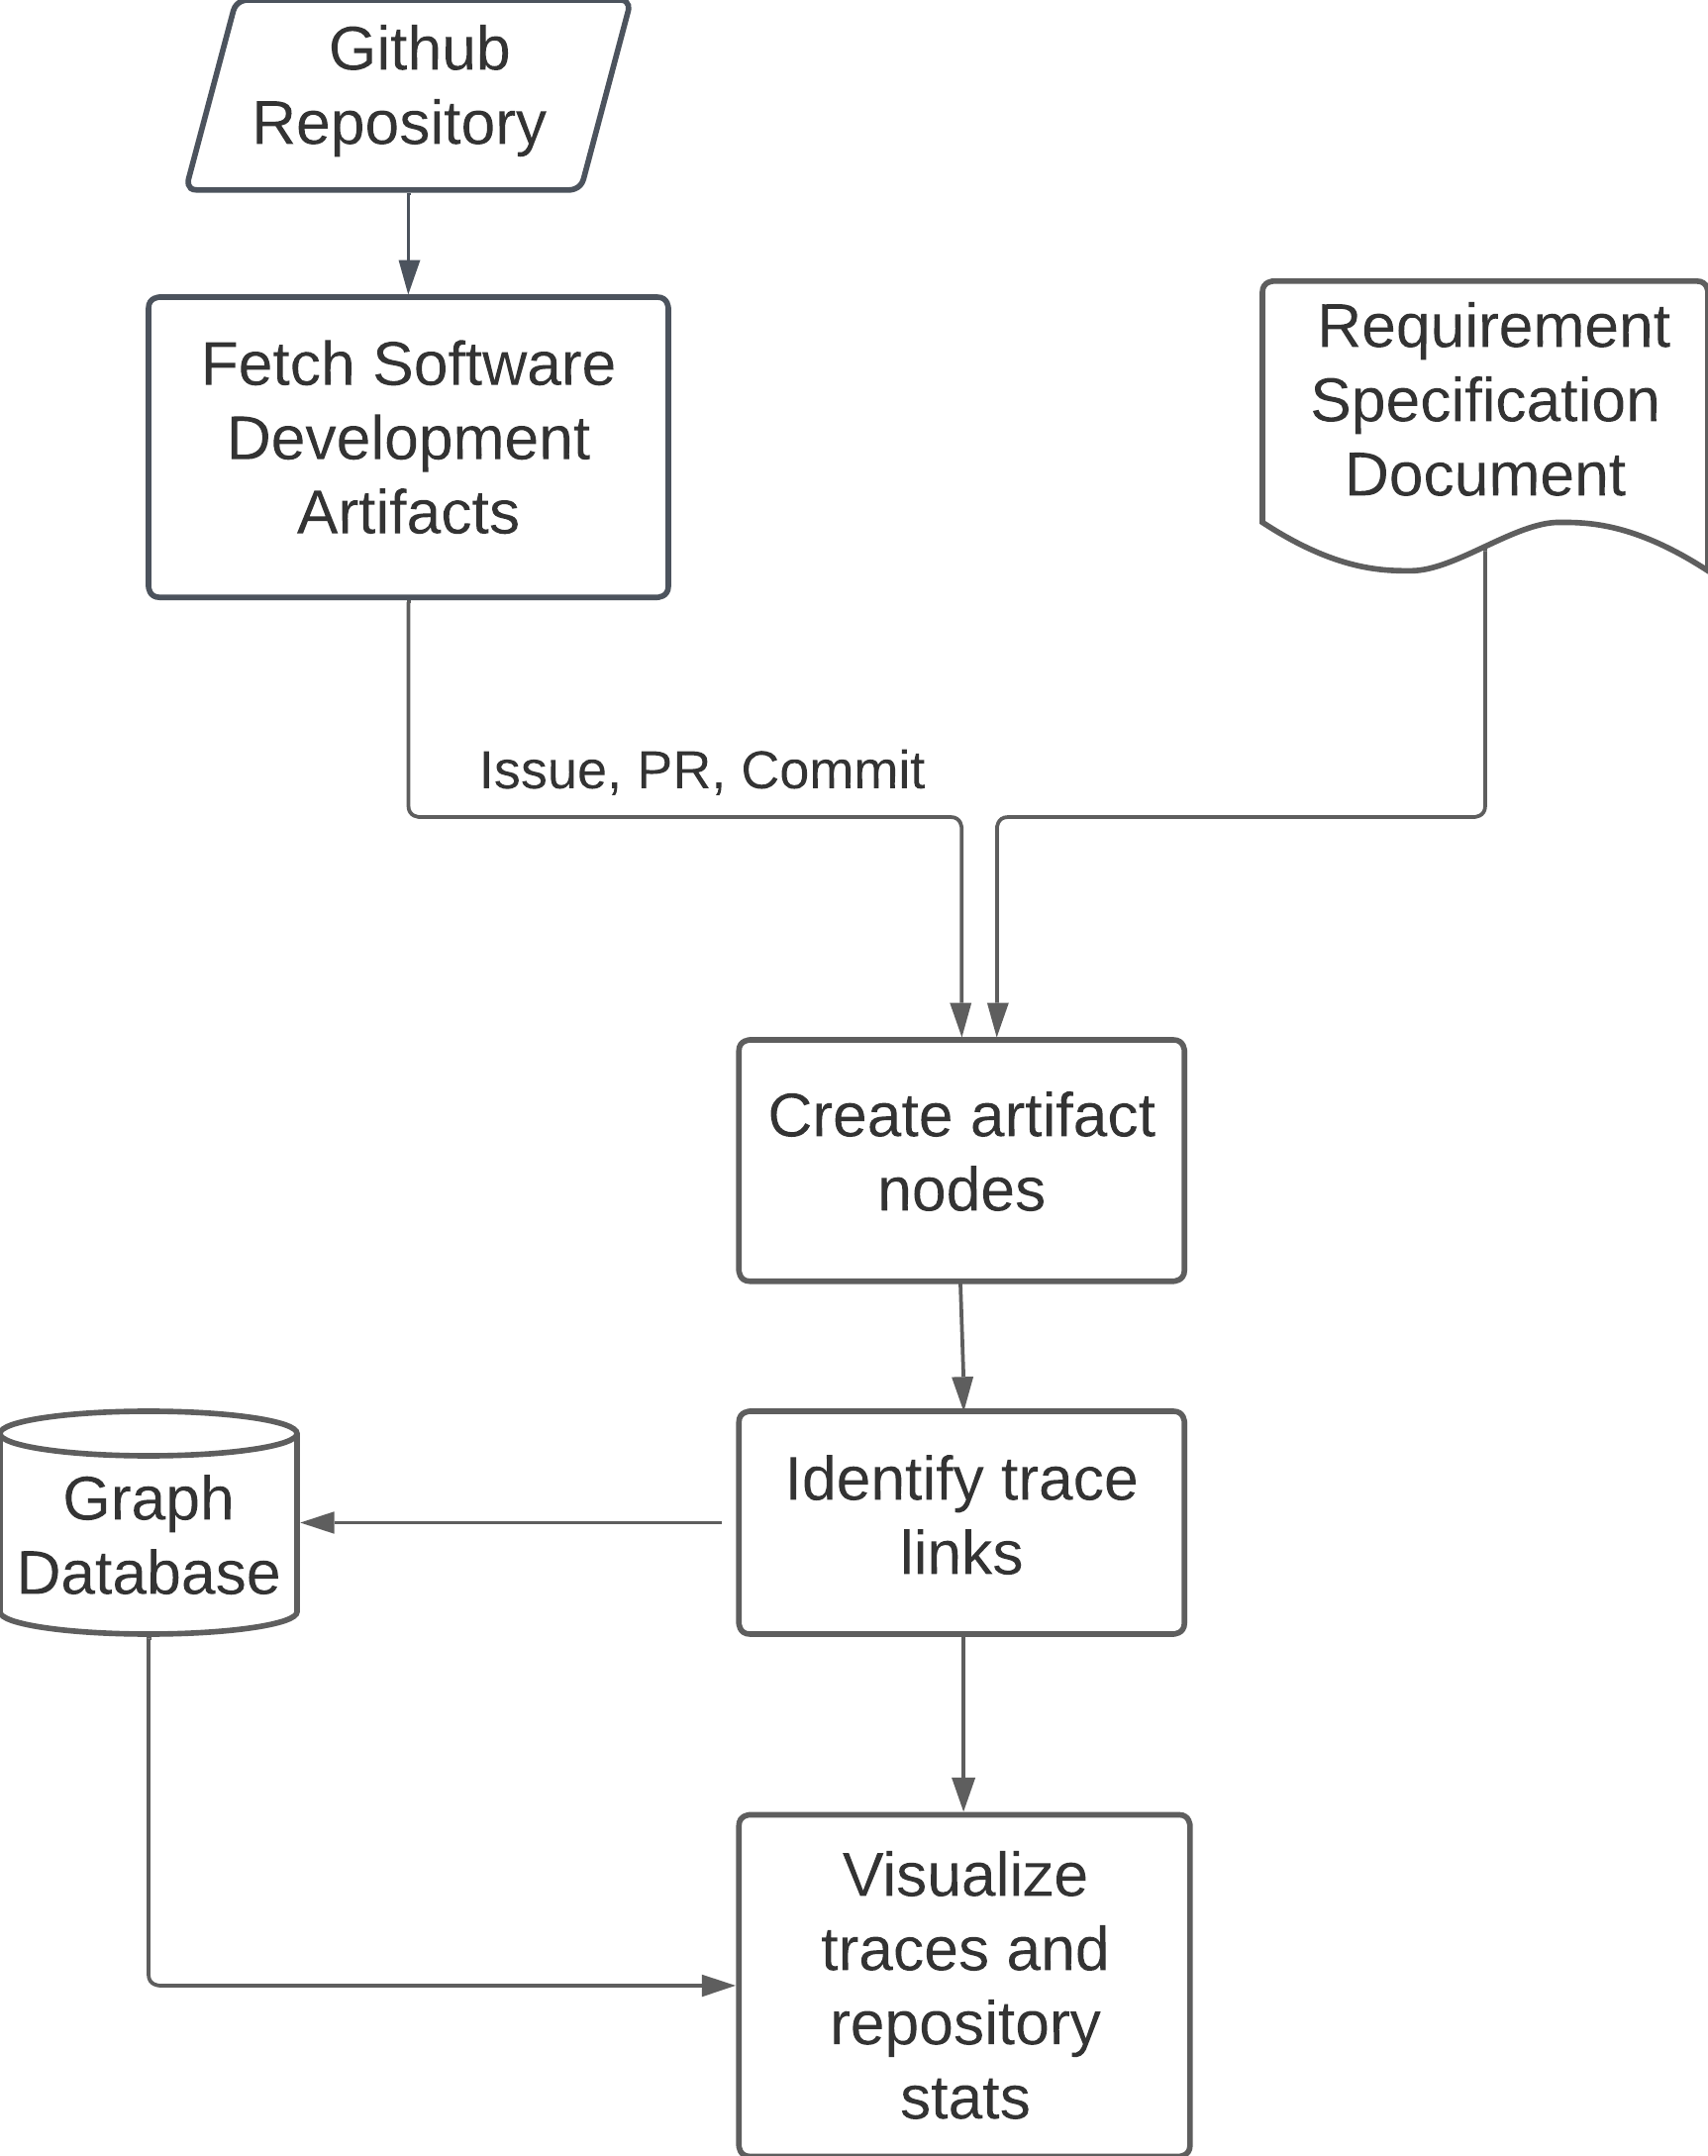
\includegraphics[width=0.45\linewidth]{figs/toolflow.png}
    \caption{Control flow of the system.}
    \label{fig:sys-flow}
\end{figure}

The tool expects a Requirement Specification Document(RSD) in the form of a text file written in natural language, along with a URL to the GitHub repository of the software project. The software development artifacts, namely Issues, PRs and Commits are fetched from the repository leveraging the GitHub API
and the requirement statements are parsed from the given RSD. This operation yields files containing information about Software Development Artifacts (SDA) and requirements, with their associated properties, such as title, description, creation and closure dates, status, and URLs. These artifacts serve as the data source for establishing trace links.

In the subsequent step, the file containing the information about SDAs and RDS are parsed to create graph nodes. At the completion of this operation, there are nodes representing each requirement and each SDA. The properties of the artifacts are stored as a property of the graph nodes. Later on, these nodes are saved into the graph database.

Furthermore, the trace links for each requirement statement are identified. The tool has three different methods implemented for trace link recovery as displayed in Figure \ref{fig:trace-methods}. The first method involves a keyword extraction, where the significant keywords from requirement specification are extracted using a custom pipeline that utilizes \textit{dependency parsing}. These keywords serve as the basis for identifying trace links between SDAs and requirements. Keyword-matching is performed on the textual data of each SDA, to capture artifacts that include the keyword as a candidate trace. The second method utilizes the TF-IDF (Term Frequency-Inverse Document Frequency) algorithm, which creates a vector for each artifact, based on the importance of the terms in their textual data. By comparing the TF-IDF vectors, the potential trace links are identified. The third method acquires word embeddings for each artifact text using a pre-trained model, creating a document vector by averaging the word embeddings, and compares these vectors to identify traces, similar to the TF-IDF vector method. 

After the identification of the trace links, the graph database is utilized to store the trace links, along with requirements and SDAs. The use of a graph database offers a scalable solution and facilitates easy retrieval of traceability data through queries. More importantly, the graphical structure of the software artifacts and the requirements provides a comprehensive visualization of the trace links.

Additionally, an interactive dashboard that visualizes the statistical information about the project and the requirements is developed. The dashboard includes various reports suitable for each kind of insight displayed, and facilitates a deeper understanding of the status and the complexity of the requirements, and provides information about the effort given to requirements during their lifetime.

\begin{figure}[htb]
    \centering
    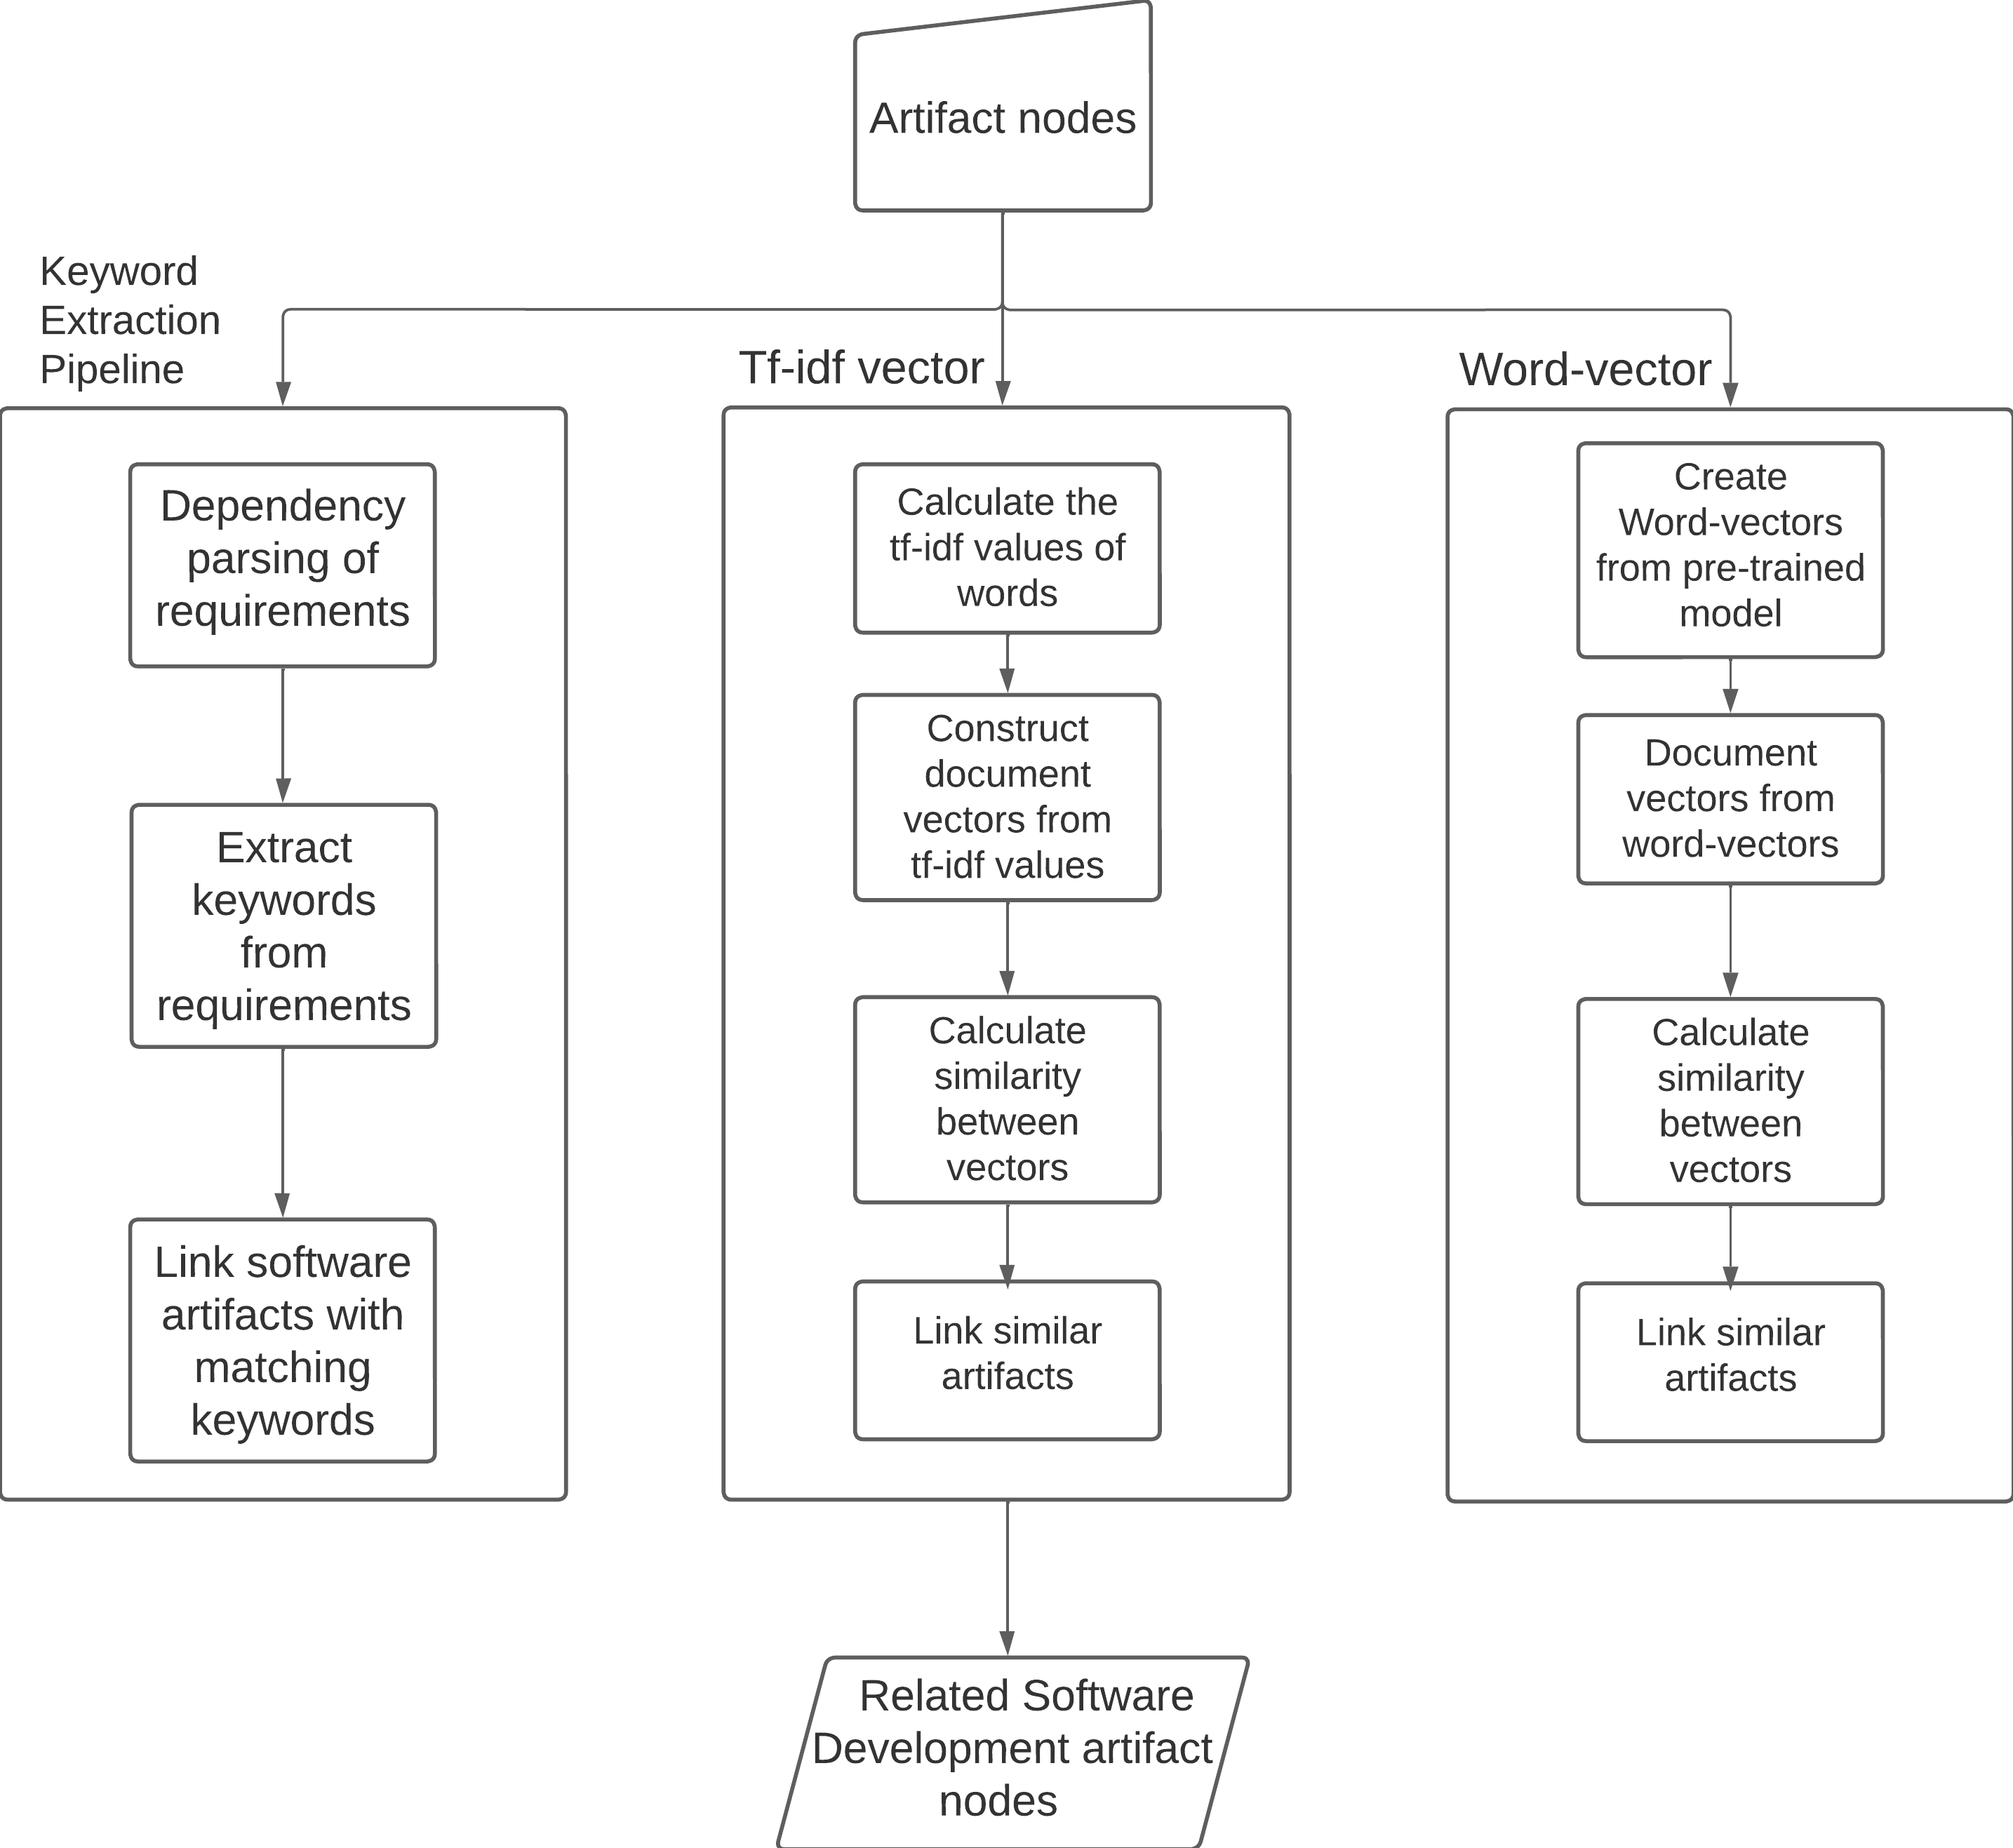
\includegraphics[width=0.6\linewidth]{figs/tracemethods.png}
    \caption{Control flow of the trace methods.}
    \label{fig:trace-methods}
\end{figure}

\subsection{Heuristics}
\label{sec:heuristics} 

\textbf{1 - Keyword Extraction}

To implement the keyword extraction method, a heuristic approach is taken, that includes several steps to extract the most relevant keywords from requirement statements. The steps of the process are as following:

\begin{itemize}
    \item Tokenization and Part-of-Speech(POS) Tagging:
        \begin{itemize}
            \item Each word of the requirement statement is tokenized.
            \item POS tagging is applied to each token. These tokens conclude information that categorizes the words as nouns, verbs, adverbs, adjectives etc.
        \end{itemize}
    \item Selecting Nouns and Verbs:
        \begin{itemize}
            \item Tokens that have \textit{noun} or \textit{verb} tag are extracted for further processing.
        \end{itemize}
    \item Dependency Parsing:
        \begin{itemize}
            \item Dependency parsing tree, which consists of dependency links is built.
            \item These links capture syntactic relationships and the dependencies between the words in a sentence.
        \end{itemize}
    \item Selecting Noun-Object and Verb-Object pairs:
        \begin{itemize}
            \item The dependency links of nouns and verbs selected in previous steps are analyzed to capture direct objects that are linked to them. 
            \item Nouns, verbs, and their corresponding objects are stored as "keywords" with labels \textit{noun-object} or \textit{verb-object}, based on the token tag. 
        \end{itemize}
    \item Selecting Prepositions and Conjunctions:
        \begin{itemize}
            \item There are indirect objects linked to nouns and verbs using prepositions(e.g. on, at, it) and conjunctions(e.g. and, or). Further analysis is applied to noun and verb tokens to capture indirect objects and build phrases.
        \end{itemize}
    \item Removal of English Stopwords:
        \begin{itemize}
            \item English stopwords, such as articles, pronouns, and common conjunctions, are removed from the tokens.
            \item This process helps to reduce noise that could arise when keyword matching is applied to software development artifacts.
        \end{itemize}
    \item Optional: Removal of Project Specific Words from Requirement Specification Documents
        \begin{itemize}
            \item Words that are frequently used in the SDAs and requirement statements, which usually are not considered as english stopwords, are also removed.
            \item However, this step is considered optional and user is expected to provide such words.
        \end{itemize}
\end{itemize}

By employing this approach, the keyword extraction method effectively captures the significant keywords from requirement specifications and prepares a base for identifying trace links. The last step of the method is to perform keyword matching using regex statements among SDAs, and record the artifacts that include the keywords as trace links. There is an example results of keyword extraction for a requirement specification down below:\\

\textit{1.3.6.1 User shall select a portion of the text for annotation.}

\textbf{Extracted keywords}: 
\begin{itemize}
    \item \textit{'verbs'}: []
    \item \textit{'verb-objects'}: ['select portion', 'select for annotation', 'select annotation', 'select text']
    \item \textit{'nouns'}: ['text', 'annotation']
    \item  \textit{'noun-objects'}: ['portion of text']\\
\end{itemize}

% Initially, part of speech(PoS) tagging and dependency parsing is applied to the requirement statement(RS). This process reveals the grammatical tags of each word and their relation with each other. Then, the verbs and nouns of the RS are inspected. 
% \begin{itemize}
%     \item Verbs and their related objects extracted as verb-object keywords.
%     \item Nouns and their compounds extracted as noun-phrase keywords.
%     \item Extra verb-object pairs extracted by inspecting conjunction links. In structures like \textit{"verb - object1 and object2"}(i.e. update username and password) verb usually has a link to the object1 and objects have conjunction link in between. Verb-object2 is extracted with this process. 
%     \item Raw verbs that does not have any of these relations extracted directly.
%     \item Raw nouns are extracted directly in any case.
% \end{itemize}

% Further, these keywords are searched among the SDAs using regular expression matching and the SDAs that have matching keywords are recorded as candidate traces. (Should i include regular expressions themselves here)

\textbf{2 - Vector based methods}

\textit{TF-IDF vectors}

To generate tf-idf vectors for each artifact(SDAs and requirements):

\begin{itemize}
    \item A corpus is established by words consisted in all SDAs and requirements, except the english stopwords.
    \item Tf-idf value of each word in the corpus is calculated. (Figure \ref{fig:tfidf})
    \item A vector for each artifact is created by the tf-idf values of words contained in their text.
\end{itemize}


\begin{figure}[htb]
    \centering
    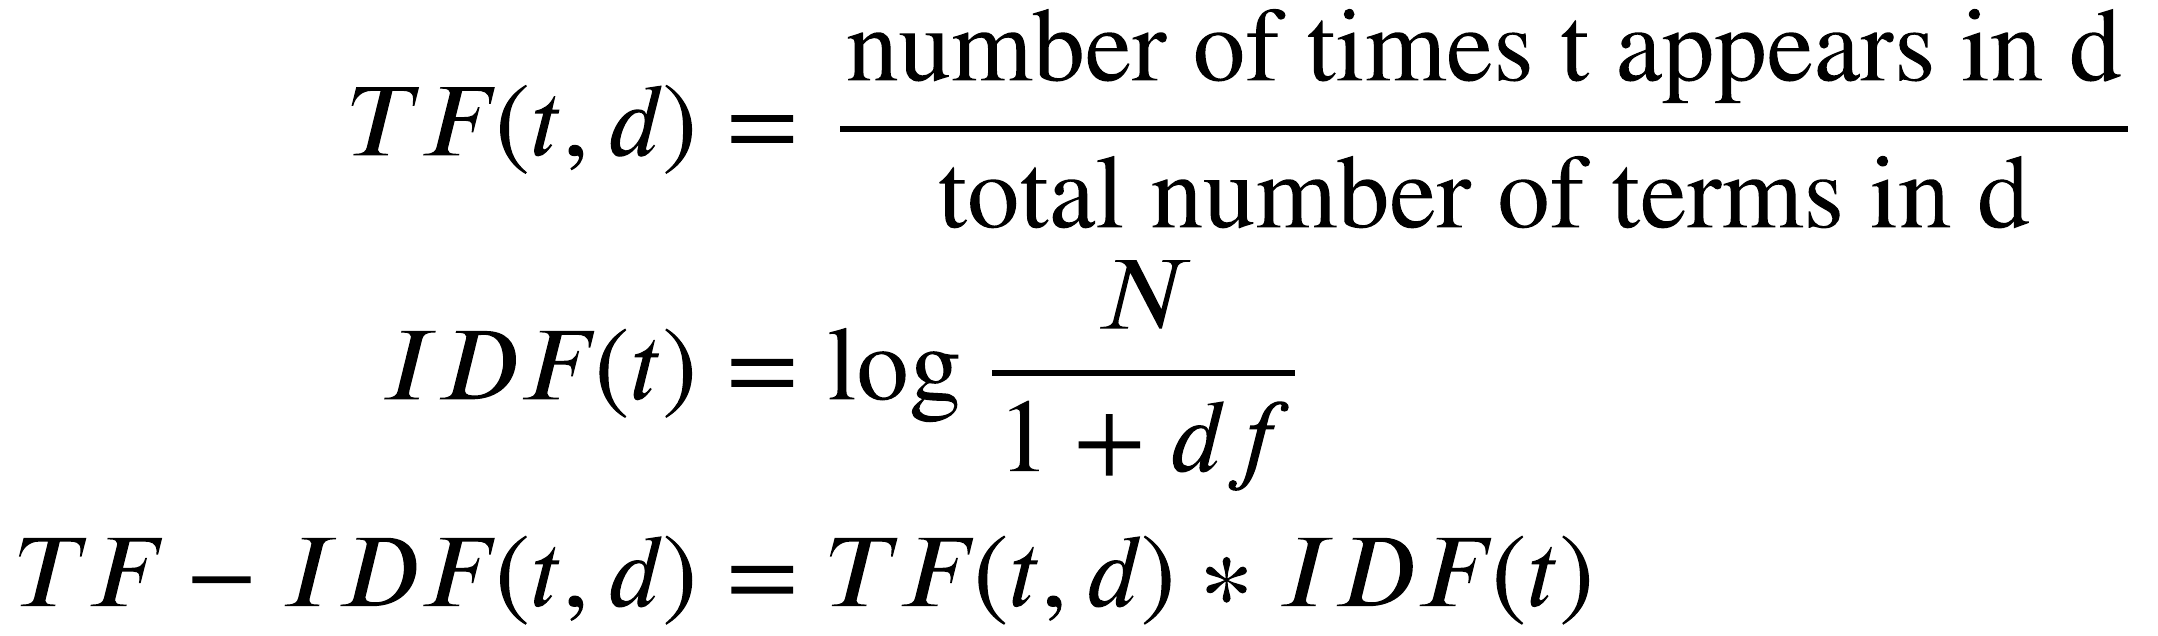
\includegraphics[width=0.75\linewidth]{figs/tfidf.png}
    \caption{TF-IDF equations.}
    \label{fig:tfidf}
\end{figure}

\pagebreak

\textit{Word vectors}

To generate word vectors for each artifact:

\begin{itemize}
    \item A pre-trained word embeddings model is utilized.
    \item The word vector for each word within an artifact text is gathered from the model.
    \item A vector for each artifact is created by averaging the word vectors contained in their text.
\end{itemize}


The last step of the vector-based methods is to check the cosine similarity of the requirement vector with every other SDA. The artifacts that have similarity above the decided threshold are recorded as candidate traces.
%\textit{Heuristic 1 - Substring Match}. Our first heuristic depends on the substring matches that can be observed among noun phrases. This process can be briefly explained as clustering noun phrases with the subset of noun phrases that contain a particular noun phrase as a substring. For example, "item label" and "item label size" noun phrases will be clustered under the "item label" key because "item label size" denotes a property of "item label". By applying this heuristic, all of these noun phrases are clustered into a set and the shortest noun phrase will represent these noun phrases. This heuristic reduces the size of the initial set of noun phrases. The reduction in the size of the initial set of noun phrases also decreases the time and space complexity of further steps of processing.

%After applying the first heuristic, we manage to cluster some of the model labels. However, there are still independent model labels. Even though the models are generated by modeling experts, modelers with different backgrounds may use different words for the same concept. For example, "shipment options" and "shipping offers" will be matched as similar noun phrases because of the high level of relatedness between the two of the noun phrases. To increase coverage of the NLP pipeline, we benefit from BERT \cite{devlin2018bert} which is a state-of-the-art deep language model. Thus, glossary extraction from models is provided by measuring the similarity of different noun phrases to each other and detecting different noun phrases that refer to a similar meaning via pre-trained sentence embeddings.

%First, noun phrases are encoded using sentence transformers which are provided by Hugging Face\footnote{https://huggingface.co} and are designed to be used with a pre-trained model. There is a variety of pre-trained sentence embedding models available for sentence embedding. We choose \textit{paraphrase-mpnet-base-v2} due to its high performance on STSbenchmark test. This sentence encoding process yields vectors that have 768 dimensions for each noun phrase. To extract similar noun phrases, pairwise cosine similarities are calculated between each noun phrase, and the symmetrical similarity matrix is obtained.




%\begin{algorithm}[htp]
%\SetAlgoLined
%\SetKwInOut{input}{Input}
%\SetKwInOut{output}{Output}
%\input{parent term P and term T}
%\output{parent term}
%parent = P\;
%term\_string = T + parent\;
%keywords = extracted keyword and probability pairs from term\_string using KEYBERT\\
%\uIf{length of keywords $>$ 1}{
%set most probable keyword as parent\\
%}
%\textbf{return} parent\;
% \caption{Heuristic 3}
%\end{algorithm}

%\textit{Heuristic 3 - Keyword Extraction}. Keyword extraction methods are mostly used for extracting the most representative n-grams from the texts. In this heuristic, lemmatized versions of both key and value are collected for each pair and concatenated into a single string. (Line 2) KeyBERT is tuned to extract unigrams from that concatenated string. (Line 3) If there exists a smaller common unit of representation for a key-value pair, both key and value are clustered under that new representation. (Lines 4 - 5)

%After applying these steps, all noun phrases extracted from the models are stored in a dictionary for reporting and visualized using an undirected graph for better understanding. Fig \ref{fig:graph} shows a sample representation extracted glossaries. Blue vertices denote matching model labels with concepts and red vertices (self-links) denote the mismatched model labels.

%\begin{figure}[htp]
%    \centering
%    \includegraphics[width=0.9\linewidth]{figs/graph.png}
%    \caption{Sample graph representation of extracted terms}
%    \label{fig:graph}
%\end{figure}

\subsection{Trace Graph}
\label{sec:tgraph}

The construction of the trace graph requires parsing the requirement specifications and the remaining software development artifacts(Issues, PRs, Commits) to create graph nodes, and executing several methods to identify trace links between them. The final step of this process is to store the nodes and the links in a Neo4j Graph Database to utilize the visualization techniques the Neo4j environment provides.

The graph nodes encapsulate following properties of the corresponding artifacts:

\begin{multicols}{2}

PR:
\begin{itemize}
\item Title
\item Body
\item URL
\item closedAt
\item createdAt
\item createdWeek
\item number
\item commentList
\item commentCount
\item commitCount
\item State
\item Text
\end{itemize}

\columnbreak

Issue:
\begin{itemize}
\item Title
\item Body
\item URL
\item closedAt
\item createdAt
\item createdWeek
\item Number
\item commentList
\item commentCount
\item State
\item Text\\
\end{itemize}

\end{multicols}

\begin{multicols}{2}    

Commit:
\begin{itemize}
\item URL
\item closedAt
\item createdAt
\item createdWeek
\item number
\item committedDate
\item oid
\item Message
\item Text
\end{itemize}

\columnbreak

Requirement:
\begin{itemize}
\item Parent
\item Number
\item Description
\item Text
\end{itemize}



\end{multicols}

The textual properties of the nodes are required for the trace identification methods to operate. In addition, the properties enable the observation of the creation/closure times, the status of the artifacts, and the access to the GitHub page they are acquired from by the URL property. Overall, these properties provide valuable traceability data, which serve as a foundation for an interactive dashboard that provides project management and requirement lifecycle analysis.

Fig. \ref{fig:tracegraph} illustrates a segment of the trace graph for a specific requirement and displays the associated trace links.

\begin{figure}[htb]
    \centering
    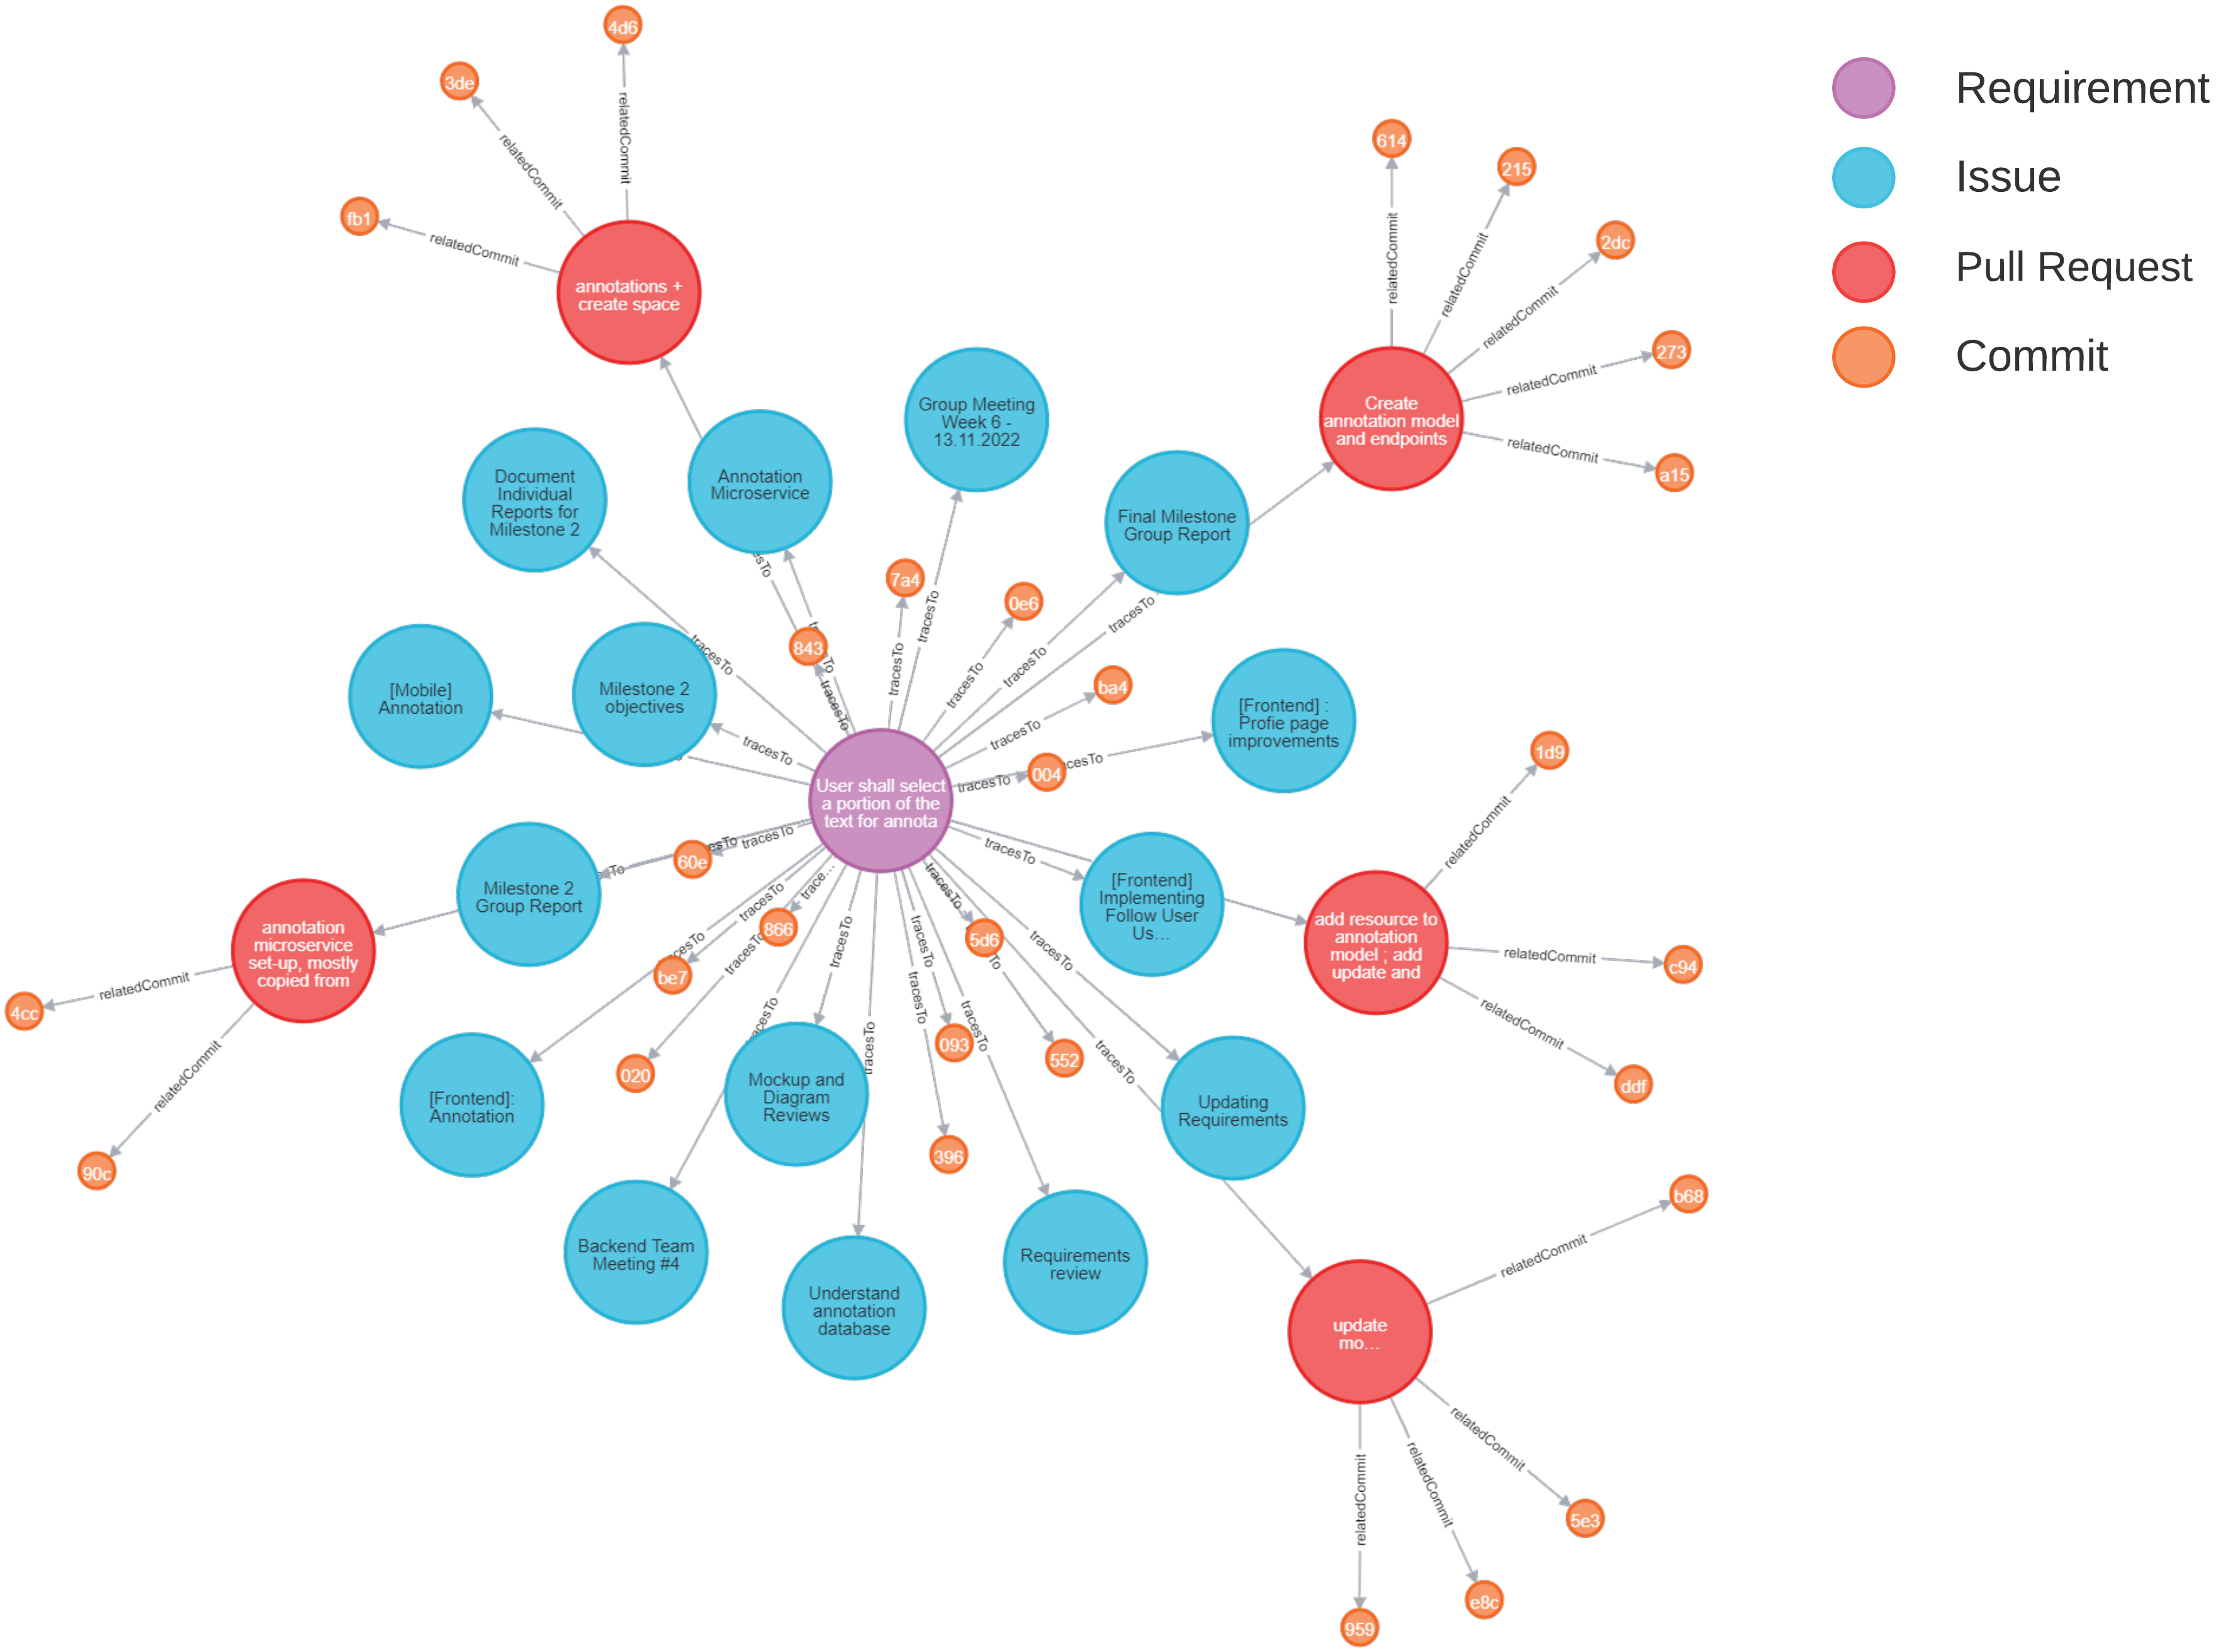
\includegraphics[width=0.75\linewidth]{figs/rawTraceGraph.png}
    \caption{A segment of the trace graph.}
    \label{fig:rawtracegraph}
\end{figure}


In Fig. \ref{fig:rawtracegraph} the trace links are organized along a time axis based on the creation date of the related software development artifacts. In this manner, the figure effectively demonstrates the lifetime of the requirement. A significant observation is that the first Pull Request related to the requirement was created in week 8, while the issues concerning the planning of the requirement were created in early stages of the development.


\begin{figure}[htb]
    \centering
    
\includegraphics[width=0.85\linewidth]{figs/traceGraph.png}
    \caption{Trace graph on a time axis.}
    \label{fig:tracegraph}
\end{figure}

% - The requirement to be examined is the root.
% - The requirement is connected to its related SDAs with \textit{tracesTo} links.
% - Pull request nodes have related commit nodes connected with \textit{relatedCommit} link.

% Who looks at trace?\\
% Trace graph can help a project manager or a developer
% Why?\\
% What can be found?


% A project manager looking at the trace graph can identify:

% \begin{itemize}
%     \item The planning phase of this requirement goes back to week 1
%     \item The implementation of this feature started at week 8
%     \item This requirement took around 13 weeks of work??
%     \item ...
% \end{itemize}

% \pagebreak

% Or in the case of a problem or a bug related to annotation, for example, a developer can view the trace of the requirement about annotation, localizing the search for the problem. Lets say the problem is about updating annotations. Looking at the trace graph, an educated guess can be made, with the information about the problem, to look at a specific pull request. For example, in our case user can view \textit{"Create annotation model"} and \textit{"... add update and delete annotation endpoints..."} nodes. Both nodes can be further observed by using the url property, reaching the github page and examining the code related to them.



\subsection{Dashboard}
\label{sec:dboard}
\\

In order to reinforce the visualization of traceability data, our research includes the development of an interactive dashboard, which offers various reports that display statistical insights. Each of these reports was carefully selected to effectively visualize the corresponding data, hence they have user-friendly designs for enhanced comprehension. Moreover, many of these reports are interactive and they allow users to trace the specific requirements, thereby enabling a more customized exploration of the traceability information.
The dashboard was implemented using Neodash technology, to provide full integrity with the traceability graph that is stored in the Neo4j database.

The first report featured in Fig. \ref{fig:barcharts} is a stacked bar chart showing the number of created Issues(in green) and PRs(in brown) for the BUcademy application. It could be observed that the highest number of created artifacts were in week 3 and week 7. The next report is another stacked bar chart that represents the number of artifacts opened and closed per week. Both of these charts are providing information about the status of development in the project lifetime and they help to identify periods of high or low development intensity and let users observe the assessment of the overall project dynamics.

The dashboard also provides static data regarding the number of open/closed issues, the number of open/merged PRs, and the average number of trace links per requirement. These statistics serve as a snapshot of the current state of the project.

\begin{figure}[htb]
    \centering
    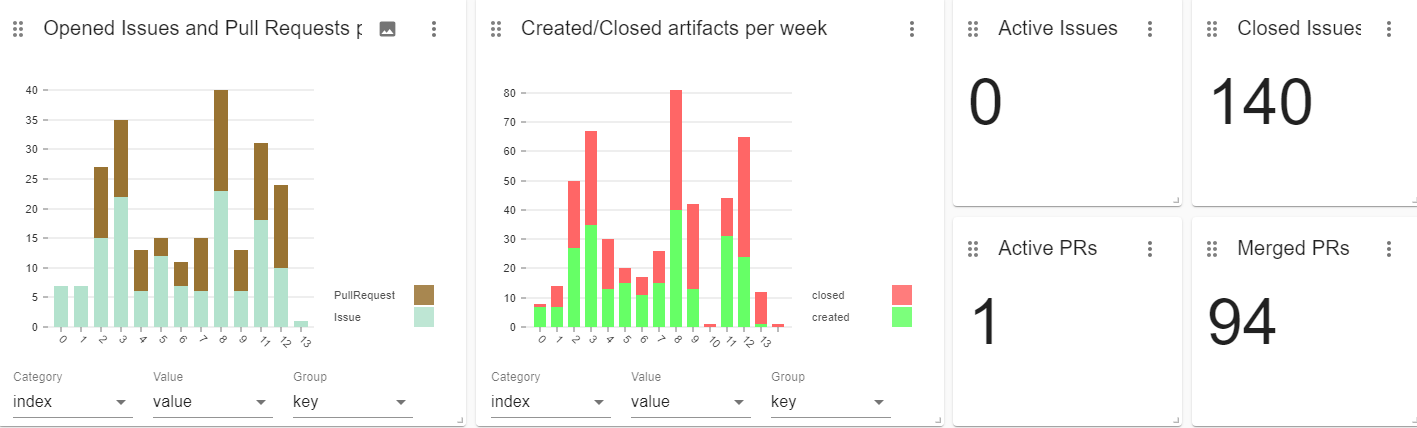
\includegraphics[width=0.9\linewidth]{figs/dashboard-barcharts.png}
    \caption{Bar charts and static data on dashboard.}
    \label{fig:barcharts}
\end{figure}

Fig. \ref{fig:linechart} continues with the line chart that illustrates the number of trace links for each requirement. By comparing the number of traces for each requirement, the report demonstrates the outliners, that could have relatively less or more traces. This comparison allows the users to observe the effort associated with each requirement since it displays the number of software development artifacts traced to them.

\begin{figure}[htb]
    \centering
    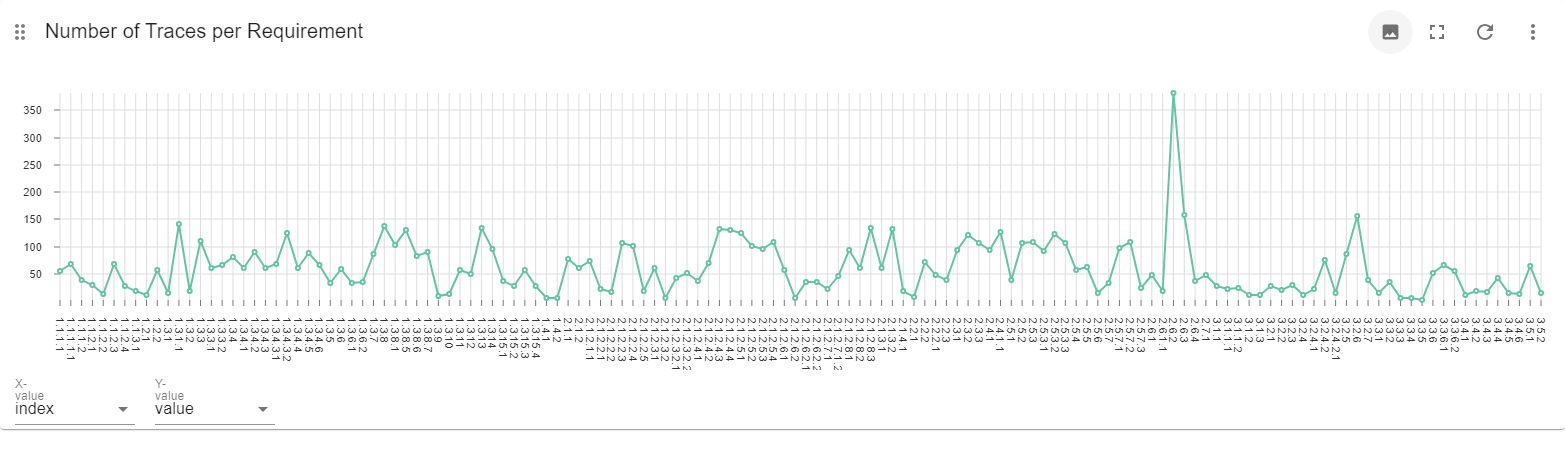
\includegraphics[width=0.9\linewidth]{figs/linechart.png}
    \caption{Line chart on dashboard.}
    \label{fig:linechart}
\end{figure}

Fig. \ref{fig:sankey} includes an example of the Sankey chart present in the dashboard that showcases the commonly traced artifacts between the chosen requirements while highlighting the strength of the trace links using the weight property. Thicker links represent a stronger relation from the requirement to the traced artifact. Thus, the chart represents the complementarity of the selected requirements.

\begin{figure}[htb]
    \centering
    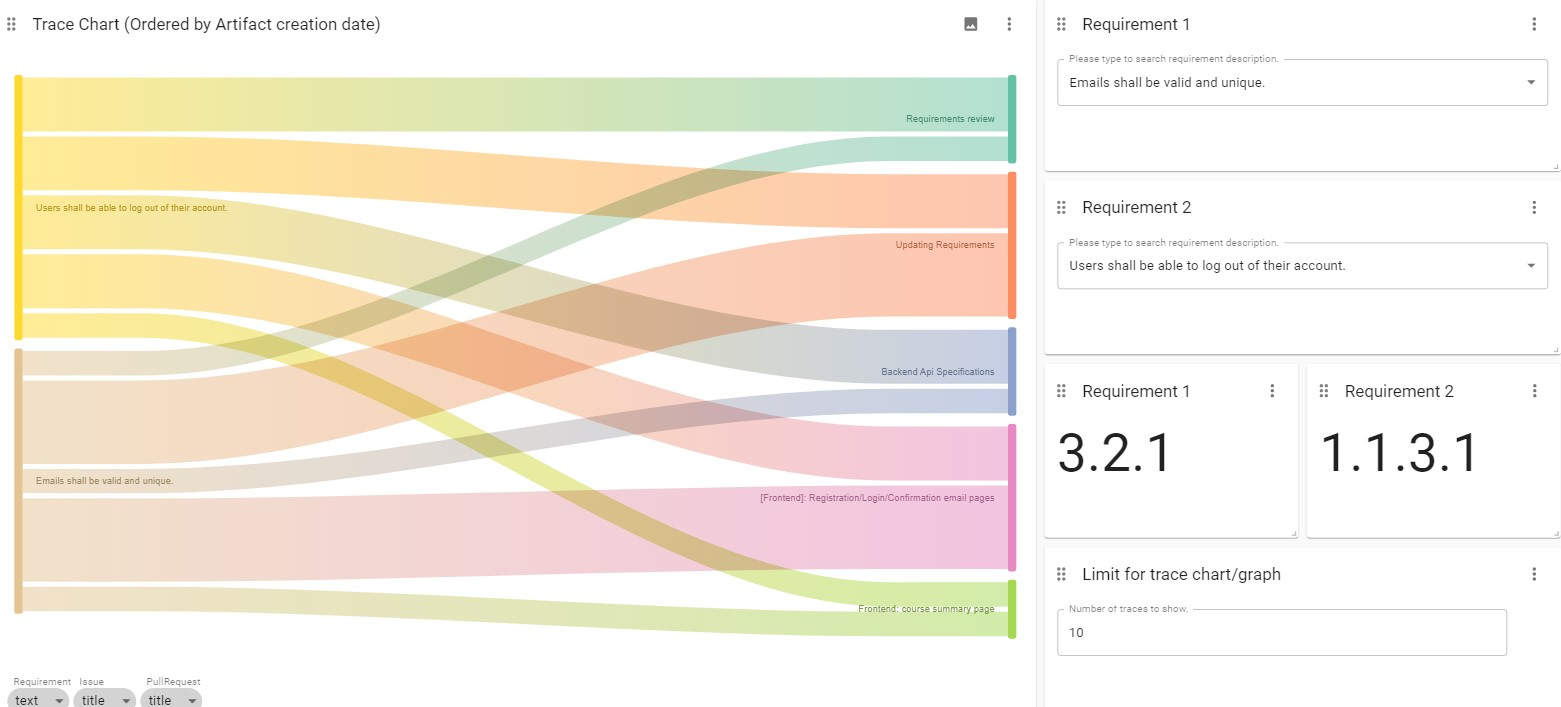
\includegraphics[width=0.9\linewidth]{figs/sankey.jpg}
    \caption{Sankey chart on dashboard.}
    \label{fig:sankey}
\end{figure}

As displayed in Fig. \ref{fig:perreq}, in addition to the generalized insights about the project status, various reports are implemented offering similar data for a specific requirement selected by the users. These include bar charts, similar to the earlier reports, tabular and graphical versions of the identified traces for the selected requirement. Overall, the current status and weekly effort given on a selected requirement are displayed in the last section of the dashboard.

\begin{figure}[htb]
    \centering
    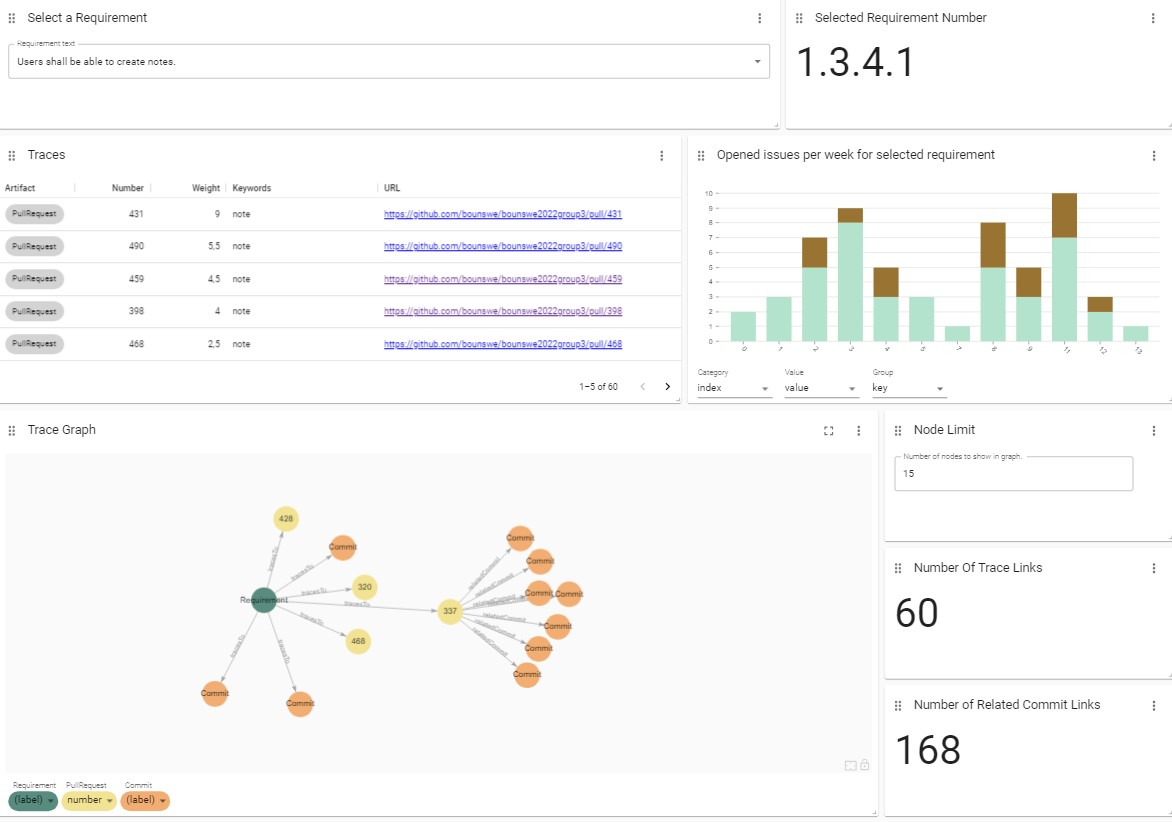
\includegraphics[width=0.9\linewidth]{figs/perreq.jpg}
    \caption{Insights for the selected requirement on dashboard.}
    \label{fig:perreq}
\end{figure}


\section{Evaluation Plan}
\label{section:evaluation}

% \begin{itemize}
%     \item Ground truth 
%     \item Experiment setup
%     \item Results
%     \item Evaluation of results
% \end{itemize}

In this section, we present the evaluation methods we performed for our tool, focusing on the accuracy of the three implemented methods for identifying trace links: keyword extraction, TF-IDF vector and word vector.

For this purpose, we designed an experiment based on a ground truth set. The information present on the set was obtained from BUcademy\cite{bounswe-bucademy} open-source project. This set consisted of eight requirement statements and software development artifacts that trace to them. These trace links were captured manually by our team. The ground truth set served as a reference to assess the accuracy of the automated methods. 

The evaluation metrics used in this experiment were recall and precision values. Recall value presents the percentage of the real traces that are recovered, while precision presents the percentage of the recovered traces that are correct. These values are calculated using the formulas below:
\\

$Recall = \dfrac{True Positives}{True Positives + False Negatives}$
\\

$Precision = \dfrac{True Positives}{True Positives + False Positives}$
\\

In the experiment, true positives indicate the trace links that are identified by the method. False negatives indicate the trace links that are not identified(missed), and false positives indicate the identified trace links that are incorrect. The results of the keyword extraction method are presented in Table I, while the results of the vector based methods are presented in Table II.


\begin{table}[htb]
\centering
\vspace{1ex}
\begin{tabular}{l l l l}
\textbf{Method} & \textbf{Recall} & \textbf{Precision}\\

Keyword extraction & \textcolor{red}{0.865} & 0.212 \\

\end{tabular}
\caption{Recall - Precision Values of Keyword Extraction Method}
\end{table}

\begin{table}[htb]
\centering
\vspace{1ex}
\begin{tabular}{l l l l l}

\textbf  & \multicolumn{2}{c}{\textbf{Word-vector}} &  \multicolumn{2}{c}{\textbf{Tf-idf vector}}\\
\textbf{Sim.Threshold   } & \textbf{Rec.} &\textbf{Prec.} &  \textbf{Rec.} &\textbf{Prec.}\\

0.05    & 1.0 & 0.043 & 0.839 & 0.121 \\
0.15    & 1.0 & 0.043 & 0.573 & 0.256 \\
0.25    & 1.0 & 0.043 & 0.244 & 0.430 \\
0.35    & 1.0 & 0.043 & 0.095 & 0.392 \\
0.45    & 0.965 & 0.071 & 0.025 & 0.125 \\
0.55    & 0.865 & 0.100 & 0.013 & 0.121 \\
0.65    & 0.294 & 0.300 & 0 & 0 \\

\end{tabular}
\caption{Recall - Precision Values of Vector-based Methods}
\end{table}

Among the tested methods, the keyword extraction method yielded the best recall-precision pair. Conversely, the performance of the vector-based methods varied significantly by the defined threshold value. For the vector-based methods, the recall value was observed as close to 1 when the threshold value was relatively low, while the precision value dropped substantially, indicating that all the necessary traces are recovered but also almost all of the SDAs have been identified as candidate traces. On the other hand, setting the threshold value too high caused the opposite effect, resulting in low recall and higher precision values. 
% Notably, the word vector method achieved the highest precision value among the results when the threshold was set to 0.25. 

In conclusion, these results indicate that each method has strong aspects, and selecting the most suitable method highly depends on the specific project structure and requirements. 



\section{Conclusions}\label{section:conclusion}

% \begin{itemize}
%     \item Observations
%     \item Threads to validity
%     \item Future Work
% \end{itemize}

In this paper, we presented a tool that automates the traceability link recovery by identifying trace links between requirements written in natural language and software development artifacts(Issues, PRs, Commits) obtained from GitHub repositories. Through the implementation of three optional methods, namely keyword extraction, TF-IDF vector and word vector, we have demonstrated the capability of identifying traceability links of our tool. We have stored the traceability data we obtained in a graph database to visualize the trace links, and supported the data with an interactive dashboard, which provides users with comprehensive statistical insights.
Our experiments on the evaluation of the tool have led us to observe that the quality and consistency of the requirement statements and the software development artifacts(SDA) significantly impact the effectiveness of the tool's capability of identifying trace links. Well-written requirement specifications that are self-explanatory and granulated lead to easier identification of its traces along with SDA which have textual data (e.g. title, description, comments) that is semantically related to the feature they implement. In this manner, our tool could be utilized for educational purposes, to assist in the improvement of writing requirement specifications.

It is important to acknowledge the threats to the validity of our study. Firstly, the absence of a ground truth set that is established by analysts may introduce bias in our evaluation process. We have prepared the ground truth set and conducted our experiments on the student projects we have participated in. Thus, we do know the capabilities of our tool and the project that we experimented on. Future work should involve validation with industry professionals and experiments designed with a wider range of projects to enhance the operating scale of our tool. 

Other several avenues for future work include providing trace links between different kinds of software artifacts, such as from Issues to PRs, to enable a deeper view of the development process. Additionally, we plan to integrate different types of requirement specifications, to accommodate diverse requirement specification document formats. Furthermore, we intend to develop a product that fetches software artifacts from various platforms such as GitLab and Jira, to improve the compatibility of the tool with different development environments that are mostly preferred within the industry. Finally, we would like to expand the variety of methods used in identifying trace links based on the needs of the users and improve the accuracy.
% by increasing the recall and precision values obtained.

In conclusion, our tool provides an automated solution for requirement traceability(RT) and enhances the management of software projects. By optimizing the time and effort required for RT and offering educational opportunities for project management, our tool contributes to the overall success of software development projects. With future development and evaluation, our study carries the potential to positively impact traceability practices.



%We present a shared collaborative modeling environment instrumented with an automated glossary extraction pipeline from model labels using state-of-the-art NLP techniques without any supervision. Our approach prevents stakeholders from spending effort on a challenging and time-consuming task of manual glossary extraction. We develop two heuristics that use pre-trained BERT models and one simple heuristic that depends on substring matching.

 %In this section, we share our plans for glossary extraction. First, we plan to conduct an experimental evaluation with human experts as we stated in Sect. \ref{section:evaluation}. Second, we plan to improve our glossary extraction heuristics' performance using human experts' feedbacks. Finally, we aim to extend our method for automated domain model extraction from model labels and employing our method as a complementary for existing systems to form a hybrid system.

\bibliographystyle{IEEEtran}
\bibliography{paper}
\end{document}